% !TEX TS-program = xelatex
% !BIB program = bibtex
% !TEX encoding = UTF-8 Unicode

\documentclass[
  oneside,
  openright,
  degree    = master,               % degree = master | doctor
  language  = english,              % language = chinese | english
  fontset   = template,             % fontset = default | template | system | overleaf
  watermark = true,                 % watermark = true | false
  doi       = true,                 % doi = true | false
]{ntuthesis}

% !TeX root = ./main.tex

% --------------------------------------------------
% 資訊設定(Information Configs)
% --------------------------------------------------

\ntusetup{
  university*   = {National Taiwan University},
  university    = {國立臺灣大學},
  college       = {管理學院},
  college*      = {College of Management},
  institute     = {資訊管理學研究所},
  institute*    = {Department of Information Management},
  title         = {構建社群媒體中品牌官方發佈內容的人氣變動模式},
  title*        = {Structuring Dynamic Popularity of Online Content from Official Brands Channels on Social Media},
  author        = {陳詩筠},
  author*       = {Shih-Yun Chen},
  ID            = {R09725037},
  advisor       = {魏志平},
  advisor*      = {Chih-Ping Wei},
  date          = {2022-07-01},         % 若註解掉,則預設為當天
  oral-date     = {2022-07-01},         % 若註解掉,則預設為當天
  DOI           = {10.5566/NTU2022XXXXX},
  keywords      = {LaTeX, 中文, 論文, 模板},
  keywords*     = {LaTeX, CJK, Thesis, Template},
}

% --------------------------------------------------
% 加載套件(Include Packages)
% --------------------------------------------------

\usepackage[sort&compress]{natbib}      % 參考文獻
\usepackage{amsmath, amsthm, amssymb}   % 數學環境
\usepackage{ulem, CJKulem}              % 下劃線、雙下劃線與波浪紋效果
\usepackage{booktabs}                   % 改善表格設置
\usepackage{multirow}                   % 合併儲存格
\usepackage{diagbox}                    % 插入表格反斜線
\usepackage{array}                      % 調整表格高度
\usepackage{longtable}                  % 支援跨頁長表格
\usepackage{paralist}                   % 列表環境
\usepackage[toc,page]{appendix}


\usepackage{lipsum}                     % 英文亂字
\usepackage{zhlipsum}                   % 中文亂字

% --------------------------------------------------
% 套件設定(Packages Settings)
% --------------------------------------------------


\begin{document}

% 封面與口試審定
% Cover and Verification Letter
\makecover                          % 論文封面(Cover)
% \makeverification                   % 口試委員審定書(Verification Letter)

% 致謝與論文摘要
% Acknowledgement and Abstract
% % !TeX root = ../main.tex

\begin{acknowledgement}

常到外國朋友家吃飯。當蠟燭燃起,菜肴布好,客主就位,總是主人家的小男孩或小女孩舉起小手,低頭感謝上天的賜予,並歡迎客人的到來。

我剛到美國時,常鬧得尷尬。因為在國內養成的習慣,還沒有坐好,就開動了。

以後凡到朋友家吃飯時,總是先囑咐自己;今天不要忘了,可別太快開動啊!幾年來,我已變得很習慣了。但我一直認為只是一種不同的風俗儀式,在我這方面看來,忘或不忘,也沒有太大的關係。

前年有一次,我又是到一家去吃飯。而這次卻是由主人家的祖母謝飯。她雪白的頭髮,顫抖的聲音,在搖曳的燭光下,使我想起兒時的祖母。那天晚上,我忽然覺得我平靜如水的情感翻起滔天巨浪來。

在小時候,每當冬夜,我們一大家人圍著個大圓桌吃飯。我總是坐在祖母身旁。祖母總是摸著我的頭說:「老天爺賞我們家飽飯吃,記住,飯碗裡一粒米都不許剩,要是蹧蹋糧食,老天爺就不給咱們飯了。」

剛上小學的我,正在念打倒偶像及破除迷信等為內容的課文,我的學校就是從前的關帝廟,我的書桌就是供桌,我曾給周倉畫上眼鏡,給關平戴上鬍子,祖母的話,老天爺也者,我覺得是既多餘,又落伍的。

不過,我卻很尊敬我的祖父母,因為這飯確實是他們掙的,這家確實是他們立的。我感謝面前的祖父母,不必感謝渺茫的老天爺。

這種想法並未因為年紀長大而有任何改變。多少年,就在這種哲學中過去了。

我在這個外國家庭晚飯後,由於這位外國老太太,我想起我的兒時,由於我的兒時,我想起一串很奇怪的現象。

祖父每年在「風裡雨裡的咬牙」,祖母每年在「茶裡飯裡的自苦」,他們明明知道要滴下眉毛上的汗珠,才能撿起田中的麥穗,而為什麼要謝天?我明明是個小孩子,混吃混玩,而我為什麼卻不感謝老天爺?

這種奇怪的心理狀態,一直是我心中的一個謎。

一直到前年,我在普林斯頓,瀏覽愛因斯坦的我所看見的世界得到了新的領悟。

這是一本非科學性的文集,專載些愛因斯坦在紀念會上啦,在歡迎會上啦,在朋友的喪禮中,他所發表的談話。

我在讀這本書時忽然發現愛因斯坦想盡量給聽眾一個印象:即他的貢獻不是源於甲,就是由於乙,而與愛因斯坦本人不太相干似的。

就連那篇亙古以來嶄新獨創的狹義相對論,並無參考可引,卻在最後天外飛來一筆,「感謝同事朋友貝索的時相討論。」

其他的文章,比如奮鬥苦思了十幾年的廣義相對論,數學部份推給了昔年好友的合作:這種謙抑,這種不居功,科學史中是少見的。

我就想,如此大功而竟不居,為什麼?像愛因斯坦之於相對論,像我祖母之於我家。

幾年來自己的奔波,做了一些研究,寫了幾篇學術文章,真正做了一些小貢獻以後,才有了一種新的覺悟:即是無論什麼事,得之於人者太多,出之於己者太少。因為需要感謝的人太多了,就感謝天罷。無論什麼事,不是需要先人的遺愛與遺產,即是需要眾人的支持與合作,還要等候機會的到來。越是真正做過一點事,越是感覺自己的貢獻之渺小。

於是,創業的人,都會自然而然的想到上天,而敗家的人卻無時不想到自己。

\end{acknowledgement}       % 致謝(Acknowledgement)
% % !TeX root = ../main.tex

\begin{abstract}

中文摘要中文摘要中文摘要中文摘要中文摘要中文摘要中文摘要中文摘要中文摘要中文摘要中文摘要中文摘要中文摘要中文摘要中文摘要中文摘要中文摘要中文摘要中文摘要中文摘要中文摘要中文摘要中文摘要中文摘要中文摘要中文摘要中文摘要中文摘要中文摘要中文摘要中文摘要中文摘要中文摘要中文摘要中文摘要中文摘要中文摘要中文摘要中文摘要中文摘要中文摘要中文摘要中文摘要中文摘要中文摘要中文摘要中文摘要中文摘要中文摘要中文摘要中文摘要中文摘要中文摘要中文摘要中文摘要中文摘要中文摘要中文摘要中文摘要中文摘要中文摘要中文摘要中文摘要中文摘要中文摘要中文摘要中文摘要中文摘要中文摘要中文摘要中文摘要中文摘要中文摘要中文摘要中文摘要中文摘要中文摘要中文摘要中文摘要

\end{abstract}

\begin{abstract*}

Abstract

\end{abstract*}              % 摘要(Abstract)

% 生成目錄與符號列表
% Contents of Tables and Denotation
\maketableofcontents                % 目錄(Table of Contents)
% \makelistoffigures                  % 圖目錄(List of Figures)
% \makelistoftables                   % 表目錄(List of Tables)
% % !TeX root = ../main.tex

\begin{denotation}[3cm]

\item[HPC]{
  高性能計算 (High Performance Computing)
}

\item[cluster]{
  集群
}

\item[Itanium]{
  安騰
}

\item[SMP]{
  對稱多處理
}

\item[API]{
  應用程序編程接口
}

\item[PI]{
  聚酰亞胺
}

\item[MPI]{
  聚酰亞胺模型化合物,N-苯基鄰苯酰亞胺
}

\item[PBI]{
  聚苯並咪唑
}

\item[MPBI]{
  聚苯並咪唑模型化合物,N-苯基苯並咪唑
}

\item[PY]{
  聚吡嚨
}

\item[PMDA-BDA]{
  均苯四酸二酐與聯苯四胺合成的聚吡嚨薄膜
}

\item[$\Delta G$]{
  活化自由能 (Activation Free Energy)
}

\item[$\chi$]{
  傳輸系數 (Transmission Coefficient)
}

\item[$E$]{
  能量
}

\item[$m$]{
  質量
}

\item[$c$]{
  光速
}

\item[$P$]{
  概率
}

\item[$T$]{
  時間
}

\item[$v$]{
  速度
}

\item[勸學]{
  君子曰:學不可以已。青,取之於藍,而青於藍;冰,水為之,而寒於水。木直中繩。輮以為輪,其曲中規。雖有槁暴,不覆挺者,輮使之然也。故木受繩則直,金就礪則利,君子博學而日參省乎己,則知明而行無過矣。吾嘗終日而思矣,不如須臾之所學也;吾嘗跂而望矣,不如登高之博見也。登高而招,臂非加長也,而見者遠;順風而呼,聲非加疾也,而聞者彰。假輿馬者,非利足也,而致千裏;假舟楫者,非能水也,而絕江河,君子生非異也,善假於物也。積土成山,風雨興焉;積水成淵,蛟龍生焉;積善成德,而神明自得,聖心備焉。故不積跬步,無以至千裏;不積小流,無以成江海。騏驥一躍,不能十步;駑馬十駕,功在不舍。鍥而舍之,朽木不折;鍥而不舍,金石可鏤。蚓無爪牙之利,筋骨之強,上食埃土,下飲黃泉,用心一也。蟹六跪而二螯,非蛇鱔之穴無可寄托者,用心躁也。—— 荀況
}

\end{denotation}
            % 符號列表(Denotation)

% 論文內容
% Contents of Thesis
\mainmatter
\chapter{Introduction}
\label{chap:1}

% !TeX root = ../main.tex
% \graphicspath{ {./images/} }
\section{Background}

With over 1.5 billion users worldwide, YouTube is currently one of the largest video-sharing platforms, where more than 500 hours of videos are uploaded per hour. It is not hard to imagine that launching videos to YouTube to promote brands and create trending topics worldwide is a common marketing strategy for businesses. YouTube is also regarded as a social media where users can create their channels and interact with other users with a "user-content-user" through a gluing layer of uploaded content opposing to traditional "user-user" interaction. Consequently, it is also reasonable for both academic and industrial to have put significant efforts into researching popularity prediction and patterns of information diffusion on YouTube.

Information diffusion describes how information is spread from one node to another in a network. Researches and observations of information diffusion are often conducted in various application domains. Examples of real-world applications include the performance of a marketing campaign or advertisement, the estimation of the dynamic popularity of online content, the prevention of an epidemic disease, the measuring of the spreading of news or rumor, the prospective impact of an idea, etc. Cascade is the basis of information diffusion. By structuring the information cascade of the information diffusion in a network, we can understand the crucial factors of a rapidly spreading information in a network and thus have the ability to predict the total population that a piece of propagation information can affect at any specific time.

The vigorous development of social media has changed the way people interact with brands. Users get information about brands through the posts or videos released to social media; further, they can express their feelings by leaving comments or simply clicking the like and dislike button under posts. As to businesses, they share content and launch marketing campaigns on social media in order to increase their brand awareness, create a positive brand association, and improve communications and interactions with their potential customers. Moreover, understanding how a brand campaign will perform can help businesses decide which marketing plan they are going to execute. For example, comparing a video having a short lifespan to a longer one, it may be suitable for some brands to choose the former one. That is to say, to release only one video that is expected to generate trending topics lasting for a long time. Therefore, it is valuable to explore the evolution of information popularity by structuring and understanding the information diffusion of online content in a social network.

% ref: The YouTube Social Network (2012)



% !TeX root = ../main.tex
% \graphicspath{ {./images/} }
\section{Motivation and Objective}

Research on popularity prediction has attracted attention in the past decades due to its essential involvement in daily life. Various methodologies are prosperously developed to predict the size of the population by structuring the cascade of information diffusion. The majority of existing research has proposed feature-based models using feature engineering approaches to extract critical factors to predict the popularity of information cascade. 

While some feature-based models are proved to efficiently explain whether features such as temporal features, user attributes, and content have significant effects on deciding the popularity, they are sometimes insufficient to figure out every possibility between features and popularity. More specifically, by simply building feature-based models, we may have ignored some important details and overlooked the relationship between factors and the outcome of information diffusion. 

Hence, we propose a model with both deep learning-based approaches and graph representation-based approaches to better identify the critical factors to the popularity evolution of videos published to YouTube official channels of brands. The objective of this paper include:

\begin{itemize}
\setlength{\itemsep}{0pt}
\setlength{\parskip}{0pt}
\setlength{\topsep}{0pt}
\setlength{\partopsep}{0pt}
    \item Predicting the overall popularity size that a brand campaign can affect in a social network at any given time by capturing the influential factors of an official published video.
    \item Accurately using graph-based approaches to model time series trends and user relationships in a complicated network.
\end{itemize}

The rest of this thesis is organized as follows:

\begin{itemize}
\setlength{\itemsep}{0pt}
\setlength{\parskip}{0pt}
\setlength{\topsep}{0pt}
\setlength{\partopsep}{0pt}
    \item We review related works of various approaches of modeling information diffusion on different social networks in Chapter \ref{chap:2}.
    \item Chapter \ref{chap:3} introduces our dataset and the proposed model structuring the dynamic popularity in a social network.
    \item The experiment details and results will be presented and summarized in chapter \ref{chap:4}.
    \item In the last section, we will discuss the contribution and the limitation in this thesis and share some insight and future work in chapter \ref{chap:5}.
\end{itemize}

% !TeX root = ../main.tex

\chapter{Literature Review}
\label{chap:2}

Recently, modeling the information cascade of information diffusion and predicting the effective population size in various domains have drawn significant attention. Hence, in this section, we introduce some of the works in YouTube, popularity prediction and information diffusion, graph neural network, and deep neural network.

% !TeX root = ../main.tex
% \graphicspath{ {./images/} }
\section{YouTube and Social Networking}

Being one of the most popular video content websites, YouTube has gained lots of attention in both academic and industrial fields. YouTube is not just a content-sharing platform but a social network with more than 1.5 billion registered users and can upload videos whenever they want. Their released YouTube Data API provides researchers easy access to YouTube video data. Many studies utilize the large-scale data of YouTube to observe and model the relationship between video attributes and video popularity. A user's content popularity can be predicted by examining user popularity in social and content facets \cite{37738}. Some studies such as \cite{10.1145/1298306.1298309} are interested in modeling the life cycle of YouTube videos that can provide supportive information to decision makers. Investigation of the social networking mechanisms and their impacts on video popularity of YouTube is also conducted in several studies \cite{4539688, 37738}. While \cite{37738} indicates that there are strong relationships between content creators, \cite{4539688} implies that videos are correlated with each other closely. Taking advantage of the massive traffic of YouTube, many brands release videos to improve their brand image and brand association \cite{Febriyantoro2020ExploringYM}. Therefore, finding influential factors of YouTube video consumption became valuable to businesses to determine which strategy is more suitable to their brand images \cite{article}.



% !TeX root = ../main.tex
% \graphicspath{ {./images/} }
\section{Popularity Prediction and Information Diffusion}

Studies focusing on modeling the diffusion of information have been popular in the few years. There are various approaches to formulating how information diffuses. Summarized by a survey \cite{2021}, information diffusion models can mainly be divided into three methods: featured-based models, generative models, and deep learning models. 

Feature-based models depend on feature engineering processes, where frequently used features containing temporal features \cite{8731564}, cascade structures \cite{8428538}, global graph relationships \cite{10.1145/2567948.2577312}, user and target data attributes \cite{8428538}, and content \cite{wu2018views}.

Many studies focus on describing the evolution of information diffusion with generative models. They usually assume that the dynamics of diffusion can be characterized by a probabilistic statistical generative model, e.g., Poisson Processes, epidemic models, and bass models. \cite{8896027} proposed a variation model of bass model to predict the dynamic popularity of a tweet from Twitter, a social media for users to share their ideas with short messages.

Deep learning models have widely developed in various domains, including population prediction studies. \cite{Wu_Mei_Cheng_Zhang_2016} proposed a model named Multi-scale Temporal Decomposition (MTD) to predict the popularity of photos on Flickr. MTD can automatically capture a photo's temporal patterns in different time scales and outperforms the other state-of-the-art models. In addition, graph neural network can be used to explore the relationships of users. \cite{cao2019popularity} proposed a graph-based model aiming at modeling the cascading effect in information diffusion by capturing the influences from users to their neighbors.
% !TeX root = ../main.tex
% \graphicspath{ {./images/} }
\section{Graph Neural Network}

Graph neural network (GNN) \cite{GNN} is a widely used deep neural network model aiming at capturing the dependence of nodes in graph-structured data. Graph data is often used to represent the network structure and interaction of a connected data set \cite{2021_Graph_Learning}, and social network data is one of the many applications of graph data. 

Some studies exploit the advantages of GNN models to model the interactions between users in social network, e.g.,  \cite{Wu_Mei_Cheng_Zhang_2016}. Except from user-item context, \cite{Wu_Mei_Cheng_Zhang_2016} develop processes to model temporal dynamics within different time scales. 

CoupledGNN proposed in \cite{cao2019popularity} contains two graph neural networks aiming at learning the interaction between nodes and the effect of information cascade. Graph learning methods are beneficial to figure out the patterns of cascade structure or global structure for popularity prediction in social networks \cite{10.1145/3331184.3331288}. \cite{10.1145/3331184.3331288} implements GNN models as a part of their proposed model which learns the representation of the cascade graph that is proved to have significantly improved the performance of predicting cascades in real-world datasets.

VaCas \cite{9155349} learns the structures and patterns of cascade graphs by integrating VAE and Bi-GRU to its graph neural network model. By developing graph learning in both node-level and cascade-level, VaCas can handle the propagation uncertainty of diffusion, capture the information cascade and predict accurately cascade size at the same time.
% !TeX root = ../main.tex
% \graphicspath{ {./images/} }
\section{Deep Neural Network}

Deep Neural Network is considered a powerful machine learning model as more and more breakthroughs and state-of-the-art results have been achieved in recent years. By constructing neurons in a deep neural network model, networks can learn non-linear relationships between input features and decompose complicated data to figure out hidden patterns \cite{DNN_2015}. Therefore, Deep learning methods are involved in various popularity prediction models for learning the representations and capturing the underlying dependencies. Graph neural network is also a kind of deep neural network. 

Since we have introduced and briefly listed several related works in the previous section, we would only share two studies related to other deep learning techniques here.

\cite{inproceedings} proposes a multimodal variational encoder-decoder (MMVED) framework to predict the popularity of videos. In this study, a long-short term memory (LSTM) decoder is implemented to be part of the decoder of MMVED for capturing temporal dynamics of popularity evolution.

DFTC is proposed in \cite{Liao_Xu_Li_Huang_Liu_Li_2019} aiming at capturing different patterns of popularity prediction in different stages of life cycles of online articles. Recurrent neural network (RNN) and convolutional neural network (CNN) techniques are adopted to DFTC to learn the temporal dynamic of popularity. In addition, hierarchical attention network is also involved in DFTC model and learn the representations of content features.


% !TeX root = ../main.tex
% \graphicspath{ {./images/} }
\section{Summary}

As deep neural networks is proved, by achieving the state-of-the-art results, to be beneficial to structure the underlying dependencies of temporal features and cascade graph, this research will focus on developing deep neural network model based on the experiments shown in previous works. We will try to integrate the advantages of feature-based models and deep learning models to construct a interpretable model which can effectively predict popularity given specific time in a social network.
% !TeX root = ../main.tex

\chapter{Methodology}
\label{chap:3}

% !TeX root = ../main.tex
% \graphicspath{ {./images/} }
\section{Problem Definition}

In this paper, we propose a neural network model to structure the pattern of videos published by official YouTube channels of brands. The model aims to precisely predict the popularity of a video at any given time after the video is published. We maintain a list of observed brands with their activated YouTube channels shown in Appendix A \cite{comparably_2021}.
% !TeX root = ../main.tex
% \graphicspath{ {./images/} }
\section{Model}

\subsection{Overview}

To reach the objective of our research, we design a prediction model shown in Fig. 1. The input sequence is a series of data, including attributes of a video, popularity of a video under the defined time scale, and channel attributes of each observed brand. Encoder layer is used to structure the patterns of input features after feature engineering processing. Prediction layer would output a sequence of predicted popularity of given video content in future timestamps.

\begin{figure}[h]
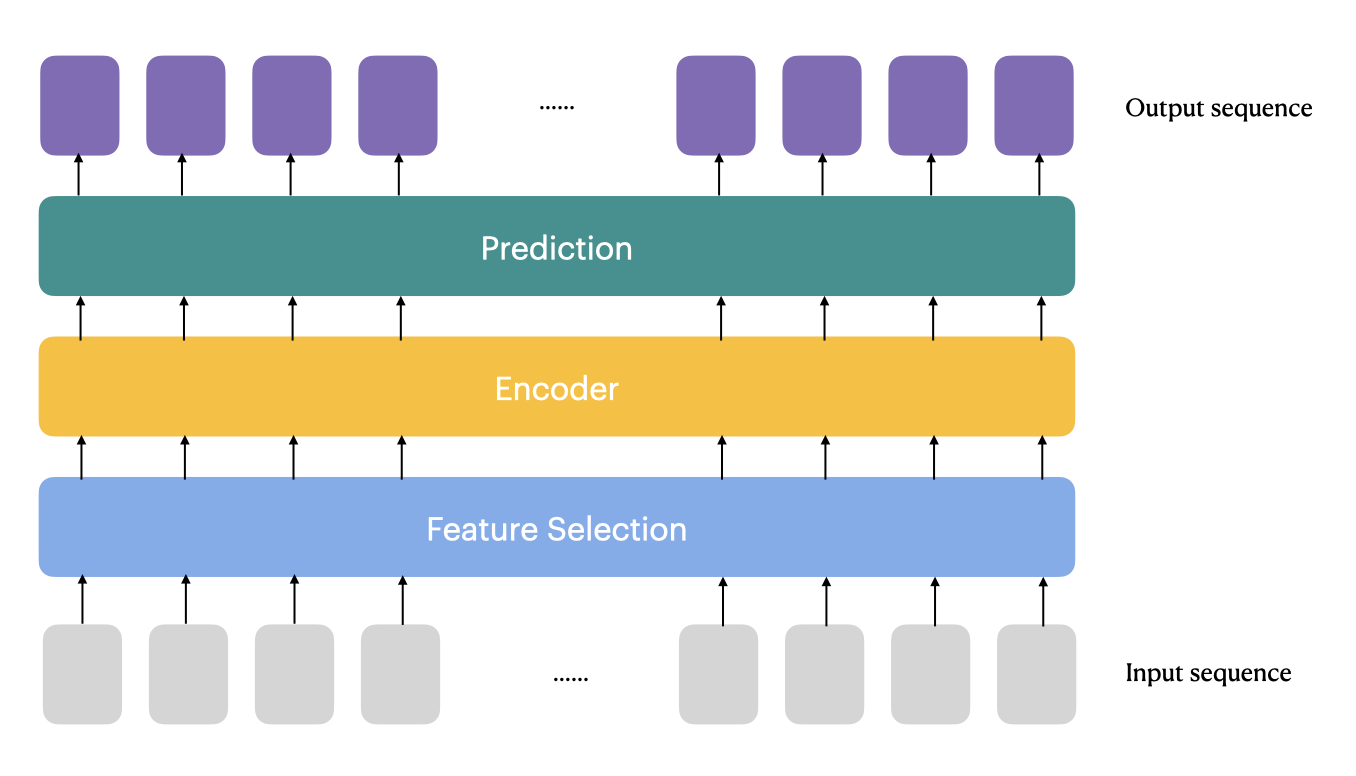
\includegraphics[scale=0.3]{figures/Proposed Model.png}
\caption{Overall framework of our proposed prediction model}
\end{figure}
% !TeX root = ../main.tex

\chapter{Experiments}
\label{chap:4}

% !TeX root = ../main.tex
% \graphicspath{ {./images/} }
\section{Dataset}

We collect Video data of YouTube of the official channels of a list of observed brands. Those brands are collected from the list of top 100 best brands and was decided by anonymous customer ratings. Customers were asked to rate the companies by several metrics: quality of the product/service, customer service, ROI, overall satisfaction, loyalty, and NPS/Net Promoter Score, and approximately 200,000 were collected in the survey.

With a list of target brands, we collect video and channel data from YouTube every day utilizing the YouTube Data API released by YouTube officially.
% % !TeX root = ../main.tex

\chapter{Conclusion}
\label{chap:5}

% 參考文獻
% References
\refmatter
\bibliographystyle{abbrv}
\bibliography{back/references}

% 附錄
% Appendices
% !TeX root = ../main.tex

\appendix{A}{Observed Brand List}
\label{appendix:a}

\begin{enumerate}
  \item Peloton
  \item Netflix
  \item Costco
  \item Chick-fil-A
  \item Amazon
  \item Apple
  \item Nike
  \item Target
  \item Google
  \item Spotify
  \item Trader Joe’s
  \item Zoom Video Communications
  \item The Walt Disney Company
  \item ROBLOX
  \item In-N-Out Burger
  \item Vans
  \item Nintendo
  \item Headspace
  \item REI
  \item Lego Group
  \item Delta Air Lines
  \item Microsoft
  \item Instagram
  \item Southwest Airlines
  \item American Eagle Outfitters
  \item Glossier
  \item Rockstar Games
  \item CHANEL
  \item LinkedIn
  \item Uniqlo
  \item Sony PlayStation
  \item Tesla Motors
  \item Starbucks
  \item NVIDIA
  \item Slack
  \item Honda
  \item Audi
  \item Red Bull
  \item Colgate Palmolive
  \item Bath & Body Works
  \item Mercedes-Benz USA
  \item Hershey Company
  \item Dunkin’
  \item Porsche
  \item Chipotle Mexican Grill
  \item BMW Group
  \item Pinterest
  \item Logitech
  \item Ritz-Carlton
  \item Shopify
  \item Crocs
  \item Gucci
  \item AMD
  \item Tiffany & Co.
  \item The Coca-Cola Company
\end{enumerate}

% \input{back/appendix02}

\end{document}
